\documentclass[11pt,a4paper]{article}
\usepackage[T1]{fontenc}
\usepackage[utf8]{inputenc}
\usepackage{lmodern,microtype}
\usepackage{amsmath,amssymb,amsthm,mathtools,bm}
\usepackage{booktabs,array,longtable}
\usepackage{graphicx,float,xcolor}
\usepackage[margin=2.05cm]{geometry}
\usepackage{enumitem,fancyhdr}
\usepackage[hidelinks,pdfencoding=auto]{hyperref}
\hypersetup{pdftitle={FIN ST342--ST356: Certified Fold Event, Symmetry Limits, and Twelve-State Observer Depth},pdfauthor={Krzysztof Żuchowski},pdfsubject={Local analytical and interval continuation of FIN Release 10.79},pdfkeywords={FIN, information, interval Krawczyk, fold, symmetry, mediator rank, Le Cam deficiency, rate distortion, refinement holonomy}}
\definecolor{proved}{RGB}{20,92,48}\definecolor{conditional}{RGB}{148,88,0}\definecolor{blocked}{RGB}{150,28,28}
\newcommand{\Proven}{\textcolor{proved}{\textbf{[PROVEN]}}}
\newcommand{\Evidence}{\textcolor{conditional}{\textbf{[STRONG NUMERICAL EVIDENCE]}}}
\newcommand{\Partial}{\textcolor{conditional}{\textbf{[PARTIAL]}}}
\newcommand{\Blocked}{\textcolor{blocked}{\textbf{[BLOCKED]}}}
\newtheorem{theorem}{Theorem}[section]
\pagestyle{fancy}\fancyhf{}\lhead{FIN ST342--ST356}\rhead{Release 10.80}\cfoot{\thepage}\setlength{\headheight}{14pt}
\setlist[itemize]{leftmargin=1.3em,itemsep=2pt,topsep=3pt}\sloppy

\begin{document}\hypersetup{pageanchor=false}
\begin{titlepage}\centering
\vspace*{1cm}{\Large Fractal Information Theory Project\par}\vspace{.8cm}
{\huge\bfseries FIN ST342--ST356\par}\vspace{.35cm}
{\LARGE Certified Fold Event, Symmetry Limits,\par}{\LARGE and Twelve-State Observer Depth\par}
\vspace{.85cm}{\large Local analytical, interval, exact finite, and bounded numerical research\par}
\vfill{\Large Krzysztof \.{Z}uchowski\par}\vspace{.2cm}
{\large Independent Researcher --- Fractal Information Theory Project\par}
{\large ORCID: 0009-0002-0909-3613\par}\vspace{.7cm}
{\large August 17, 2026\par}\vspace{.2cm}{\large Release 10.80\par}\vfill
\begin{minipage}{.92\textwidth}\small
\textbf{Repository snapshot.} Audited tracked base:
\texttt{bb540a767e210a5a3bf816e4868e7bcefbac3872}. The working tree contains
uncommitted research artifacts; the accompanying SHA-256 ledger fixes this release packet.

\medskip\textbf{License.} CC BY 4.0. \quad \textbf{Language.} English. \quad
\textbf{Resource type.} Preprint and executable reproducibility package.
\end{minipage}\end{titlepage}
\hypersetup{pageanchor=true}\pagenumbering{roman}

\begin{abstract}
Programs ST342--ST356 continue the local FIN research program after Release 10.79. Two
principal gaps are closed. First, the certified local coexistence bracket is narrowed from
width $5\times10^{-3}$ to $2\times10^{-8}$: outward endpoint objective intervals have
opposite signs and one parametric Krawczyk tube contains a unique positive reflection-even
stationary root across the full bracket. Second, the former numerical spinodal candidate is
upgraded to a full 17-variable interval event certificate. The augmented
stationarity--nullvector--normalization system has a unique root in the declared box, and
the stationary Jacobian has exactly a one-dimensional kernel there. Conventional fold
transversality coefficients remain point-certified only, so the claim is deliberately
``certified fold event'', not a global bifurcation diagram.

A new obstruction explains why global closure remains difficult. $D_{12}$ invariance maps
minimizers into finite orbits but does not force them into reflection-fixed subspaces: the
open dense simplex stratum is eleven-dimensional and has trivial stabilizer. A 173-start
audit continues to find only the localized reflection orbit at $g=4$, but this remains
strong numerical evidence. Coupling spectrally truncated conservative mediators to the
simplex shows that covariance permits ranks $1,3,5,7,9,11$; rank seven is the first at which
a pure vertex beats the uniform state exactly at $g=4$, and is also the first numerically
localizing truncation.

The 12-state permutation-covariant confusion family admits an exact Le Cam depth:
fine-to-coarse deficiency is zero and reverse deficiency is the difference of confusion
errors. A strict-heat conditional Markov source yields an exact entropy rate and a numerical
two-symbol rate--distortion curve. Two-cycle refinement complexes have two independent
gauge-invariant holonomies, and multilevel clock errors separate into cancelling common
calibration gauge and accumulating differential drift. No strict source for the active
coupling or stabilizer coefficients, global physical vacuum, selector, absolute unit, time
arrow, spacetime, apparatus, independent events, legacy-role transfer, Standard Model,
gravity, $L_{\rm total}$, or Theory-of-Everything closure is claimed.
\end{abstract}
\tableofcontents\newpage\pagenumbering{arabic}

\section{Scope and proof discipline}

The strict finite operator used in this batch is
\[
A=sI-W,\qquad W_{xx}=0,\qquad
W_{xy}=K_{\rm strict}(d(x,y))\quad(x\ne y),
\]
with $A\mathbf1=0$ and $A\succeq0$. This explicit diagonal convention is essential: the
quoted row sum $s=1.660307278766099$ belongs to the off-diagonal $W$.

The legacy ontological kernel remains an intermediate bridge object. No physical legacy
role is silently transferred to the strict kernel. The internal ontology---the nadsoliton
itself as primordial fractal information in a solitonic state, followed by light, matter,
and an emergent observer---is preserved as project context but is not used to prove the
finite theorems below.

\Proven{} marks exact analysis or outward interval certification. \Evidence{} marks
reproducible floating computation. \Partial{} marks a missing global, continuum, or source
step. \Blocked{} marks evidence that cannot be generated locally.

\section{Executive result ledger}
\small
\begin{longtable}{p{.065\textwidth}p{.20\textwidth}p{.64\textwidth}}
\toprule Program&Status&Result\\\midrule\endhead
ST342&\Proven&Local coexistence is certified in a width-$2\times10^{-8}$ bracket.\\
ST343&\Proven&Unique root of the full 17D augmented event system; stationary kernel dimension exactly one.\\
ST344&\Proven&Symmetry alone cannot reduce all global minimizers to fixed-point subspaces.\\
ST345&\Evidence&All 173 starts support the localized reflection orbit at $g=4$; no global theorem.\\
ST346&\Proven{}+\Evidence&Rank seven is the first exact vertex threshold and first numerical localization among covariant modal mediators.\\
ST347&\Proven&The spectral-energy subalgebra has 21 quartic and 56 sextic basis monomials; all 77 coefficients remain free.\\
ST348&\Proven&Zero belief memory can coexist with nonzero Chernoff pressure derivative; contraction alone cannot close the derivative tail.\\
ST349&\Partial&Anisotropic widths improve the outer-cube pass count to 34/40, but six sections remain uncertified.\\
ST350&\Proven{}+\Evidence&Finite dual support and finite threshold-band structure are analytic; numerical grid endpoints remain uncertified.\\
ST351&\Proven&A two-cycle refinement complex carries two independent gauge-invariant holonomies.\\
ST352&\Proven&Exact Le Cam deficiency for the 12-state symmetric confusion family.\\
ST353&\Proven&Matching $r\sigma^2/N$ recovery bounds in a declared spectral Gaussian experiment.\\
ST354&\Proven{}+\Evidence&Strict heat supplies a conditional Markov law and exact entropy rate; two-symbol rate--distortion is numerical.\\
ST355&\Proven&Common scale gauge cancels while differential clock error accumulates by explicit products.\\
ST356&\Blocked&No independently registered raw-event packet exists.\\
\bottomrule
\end{longtable}\normalsize

\section{ST342: a $2\times10^{-8}$ coexistence bracket}

For reflection-even probabilities represented by seven orbit values $q_i$, the stationary
equations at supplied active coupling $g$ are
\[
\log(12q_i)+1-g(Bq)_i+\lambda=0,
\qquad q_0+2\sum_{i=1}^{5}q_i+q_6=1.
\]
The new interval endpoints are
\[
g_- =2.902496471747767,\qquad
g_+=2.9024964917477667.
\]
At $g_-$, the complete objective enclosure is
\[
[1.11419\times10^{-9},\,1.23114\times10^{-8}],
\]
whereas at $g_+$ it is
\[
[-1.23114\times10^{-8},\,-1.11419\times10^{-9}].
\]
Both endpoint roots are unique in their outward boxes. A coordinatewise parametric
Krawczyk tube contains a unique positive root for every $g\in[g_-,g_+]$, with minimum
inclusion margin $9.9883\times10^{-8}$.

\begin{theorem}[narrow certified local coexistence]
The declared positive reflection-even branch has at least one point in $[g_-,g_+]$ at
which its objective equals the uniform-state objective.
\end{theorem}

\begin{figure}[H]\centering
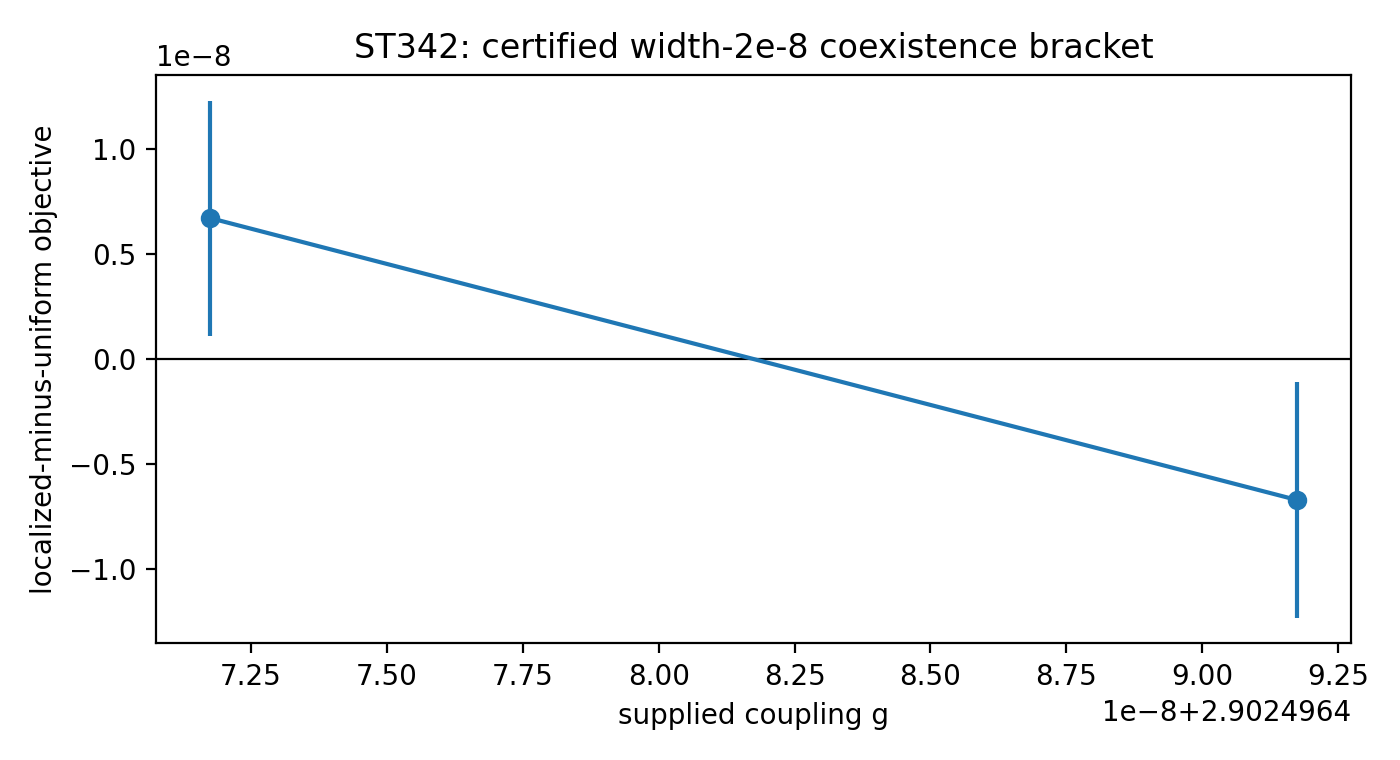
\includegraphics[width=.73\textwidth]{FIN_ST342_ST356_Figures/st342_narrow_crossing.png}
\caption{Outward endpoint objective intervals in the certified coexistence bracket.}
\end{figure}

This is a $250{,}000$-fold width improvement over ST327. It still does not establish that
the branch is globally minimizing, that the crossing is unique, or that $g$ is internally
sourced.

\section{ST343: full interval certification of the fold event}

Let $x=(q_0,\ldots,q_6,\lambda)$ and define
\[
\mathcal F(x,g,v)=
\begin{pmatrix}
F(x,g)\\ D_xF(x,g)v\\ (\langle v,v\rangle-1)/2
\end{pmatrix}\in\mathbb R^{17}.
\]
The previous floating candidate was at $g\approx2.66490805100556$. ST343 evaluates all
17 residuals and the complete $17\times17$ Jacobian with outward interval arithmetic on a
coordinate-radius $10^{-8}$ box. The Krawczyk image lies strictly inside, with minimum
component margin $9.9988863\times10^{-9}$.

\begin{theorem}[certified one-null-direction event]
The augmented system $\mathcal F=0$ has exactly one root in the declared 17D box. At that
root $D_xF$ has rank exactly seven and hence a one-dimensional kernel.
\end{theorem}

The upper rank bound follows from the certified nonzero normalized nullvector. For the lower
bound, the second-smallest singular value at the center is $3.38062$, while the paid
Frobenius perturbation bound over the box is below $7.1\times10^{-5}$, leaving rank-seven
margin $3.38055$.

The conventional point transversality diagnostics are
\[
w^TF_g\approx-0.3572266,\qquad
w^TF_{xx}[v,v]\approx0.2753332.
\]
They strongly support a simple saddle-node fold, but were not enclosed as intervals in this
batch. Accordingly the theorem certifies the event and nullity, not the entire local normal
form, dynamic stability, or global branch diagram.

\section{ST344--ST346: global symmetry limit and modal localization}

The variational objective is invariant under the 24-element dihedral group $D_{12}$. This
does not imply that every minimizer is reflection-even.

\begin{theorem}[fixed-symmetry reduction no-go]
The union of nontrivial $D_{12}$ fixed-point subspaces has empty interior in the
11-dimensional probability simplex. Its complement is open and dense and consists of
trivial-stabilizer points with 24-element orbits. Hence symmetry alone cannot reduce the
complete global minimization problem to reflection-fixed subspaces.
\end{theorem}

An explicit witness is the normalized positive vector with entries proportional to
$1,2,4,\ldots,2^{11}$: all entries are distinct, so no nonidentity dihedral permutation
fixes it. Fixed-subspace searches remain legitimate for finding symmetric critical points;
they are not an exhaustive global certificate.

ST345 therefore performs a falsification audit rather than claiming a proof. Across 173
uniform, vertex-biased, and random starts at $g=4$, the best objective is
$-0.84519850768$, the largest probability is $0.99020346$, and the minimum reflection
defect is below $10^{-7}$. Every best basin is numerically $D_{12}$-equivalent to the
localized reflection orbit. This is compelling evidence, but ST344 explains why it is not
enough.

For the mediator study, let $A_m$ retain complete degenerate spectral blocks in descending
eigenvalue order. Dihedral covariance permits only ranks
\[
1,3,5,7,9,11.
\]
The pure-vertex energy crosses the uniform energy at
\[
g_{E,m}=\frac{2\log12}{\operatorname{tr}(A_m)/12}.
\]
The values decrease from $25.4625$ at rank one to $2.99331$ at full rank. Rank seven is the
first with $g_{E,m}<4$, namely $g_{E,7}=3.90777$, and is also the first truncation whose
multistart optimum localizes numerically.

\begin{figure}[H]\centering
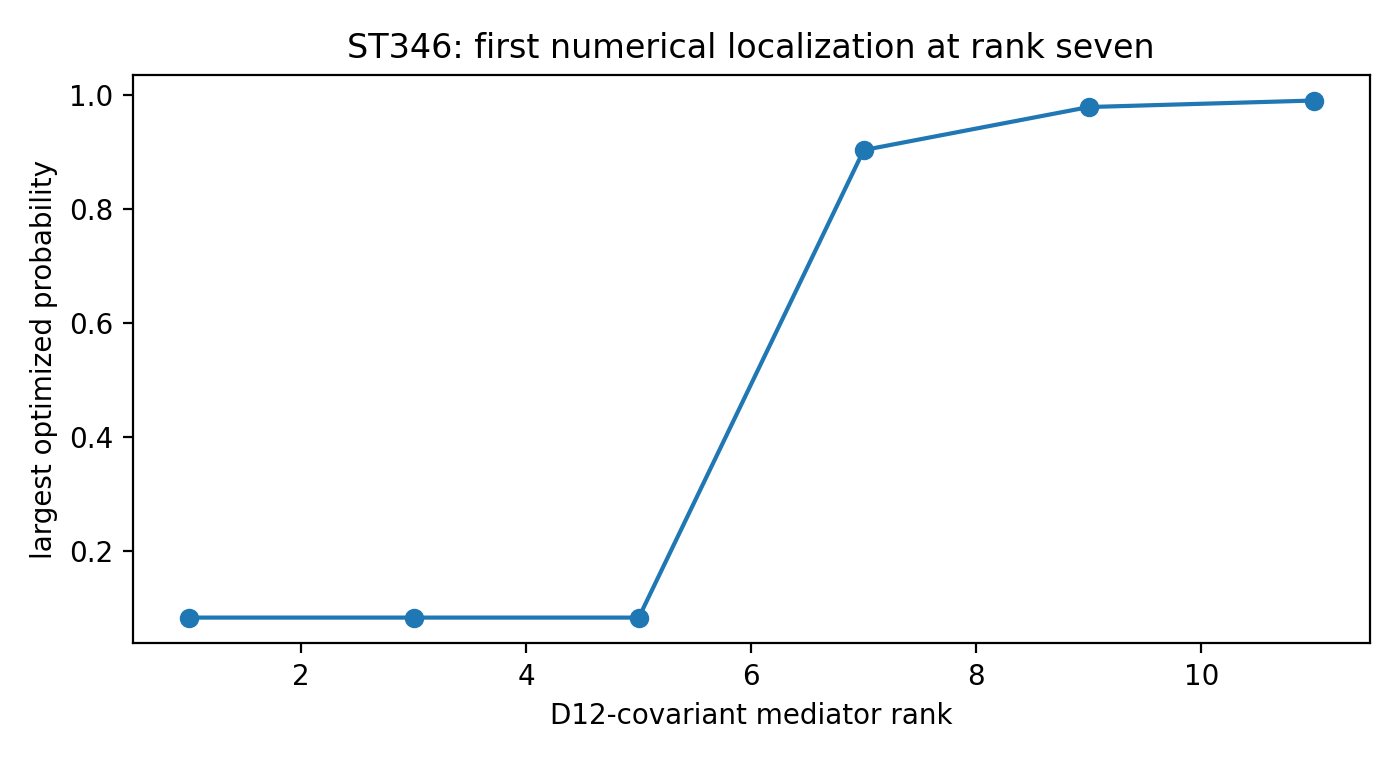
\includegraphics[width=.73\textwidth]{FIN_ST342_ST356_Figures/st346_modal_localization.png}
\caption{Uniform behavior through rank five and the first localized optimum at covariant rank seven.}
\end{figure}

Thus at least seven conservative hidden directions are needed before this particular
simplex model can energetically prefer a vertex at $g=4$. The result does not source rank,
$g$, or a physical hidden system.

\section{ST347--ST350: invariants, pressure derivatives, and continuum design}

Write $E_k(q)=\|P_kq\|^2$ for the six positive real modal energies. Within the explicitly
declared spectral-energy subalgebra, quartic invariants are $E_iE_j$ and sextic invariants
are $E_iE_jE_k$.
\begin{theorem}[spectral-energy invariant count]
The quartic basis has $\binom{7}{2}=21$ monomials and the sextic basis has
$\binom{8}{3}=56$. The strict operator distinguishes weighted combinations such as
$\langle q,Aq\rangle^2$ and $\langle q,Aq\rangle^3$, but does not choose the 77 general
real coefficients or their signs.
\end{theorem}
This scoped theorem is not a Molien classification of the full $D_{12}$ invariant ring;
phase-sensitive invariants can lie outside the modal-energy subalgebra.

ST348 proves that filter contraction cannot, by itself, close the Chernoff derivative
problem. Consider one-state i.i.d. experiments
\[
P=(0.9,0.1),\qquad Q=(0.6,0.4).
\]
Their belief-memory contraction is exactly zero, yet at $s=1/2$ the normalized per-symbol
pressure derivative is $0.0221383\ne0$. A valid all-depth theorem must therefore control
the normalized multiplicative transfer weights, not only belief forgetting.

ST349 assigns coordinatewise half-widths from adjacent ST298 sections. The resulting
anisotropy is real: 34 of 40 rigorous outer-cube tests pass, compared with 26 of 40 in the
isotropic ST333 attempt. Six failures remain. This is useful method diagnosis: the next
implementation must rotate coordinates into one longitudinal tangent and seven transverse
directions rather than intervalize a large axis-aligned hull.

For ST350, finitely many response times $t_j$ and one heat budget give a continuum linear
program. Its dual uses finitely many nonnegative time weights $\alpha_j$ satisfying
$\sum_j\alpha_j=1$ and one heat price $\nu\ge0$. The primal selector is determined by the
sign of
\[
\Theta(\mu)=\sum_j\alpha_j d_{t_j}(\mu)-\nu h(\mu).
\]
On a compact positive spectral interval, a nonzero analytic $\Theta$ has finitely many
zeros, hence finitely many threshold bands. The 250-, 500-, and 1000-point grids all find
two selected bands (four entry/exit transitions) and value near $1.27633$; exact continuum multipliers and endpoints remain
uncertified.

\section{ST351--ST353: scale cohomology and quantitative observer depth}

For a connected refinement graph, logarithmic edge calibrations form one-cochains and
vertex recalibrations are coboundaries. Therefore
\[
\dim H^1=E-V+1.
\]
The square-with-diagonal test complex has $V=4$, $E=5$, and two independent cycle
holonomies. Direct vertex recalibration leaves both invariant to below $10^{-15}$. This
generalizes the one-cycle ST335 result without assigning physical scale curvature to FIN.

Let $C_e$ be the 12-state permutation-covariant confusion channel with correct-label
probability $1-e$ and each incorrect label probability $e/11$.
\begin{theorem}[exact twelve-state observer depth]
For $0\le e_f\le e_c\le11/12$,
\[
\delta(C_{e_f},C_{e_c})=0,
\qquad
\delta(C_{e_c},C_{e_f})=e_c-e_f.
\]
\end{theorem}
The finer experiment simulates the coarser by an additional symmetric confusion channel.
Conversely, group-twirling cannot worsen worst-row total variation and reduces every
candidate postprocessing to the one-parameter covariant family; identity is the boundary
closest to the finer target. Full 144-variable stochastic LP replays agree with the formula
to $5\times10^{-16}$ for four test pairs.

For a known $r$-mode fiber in a Gaussian sequence experiment with orthonormal design,
$N_c$ independent counts and noise $\sigma$, least squares achieves
\[
\mathbb E\|\widehat B-B\|^2=\frac{r\sigma^2}{N_c}.
\]
The Gaussian translation minimax lower bound matches it. This is a sharp conditional result
and clarifies the benefit of spectral restriction. It is not a detector model: known modal
support, Gaussian noise, orthonormal design, and independence are premises.

\section{ST354--ST356: strict-heat compression, clock drift, and evidence stop}

At supplied $\tau=0.5$, the strict heat kernel
\[
P_\tau=e^{-\tau A}
\]
is strictly positive and doubly stochastic; its smallest entry is $0.0107821$. With uniform
stationary distribution it defines a conditional, operator-generated 12-state Markov
source. Its exact entropy rate is the common row entropy,
\[
h(P_\tau)=2.6057354210\quad\text{bits per symbol}.
\]
This is materially closer to FIN than the binary source used in ST338. A two-symbol
Blahut--Arimoto computation gives the conditional Hamming rate--distortion curve below.

\begin{figure}[H]\centering
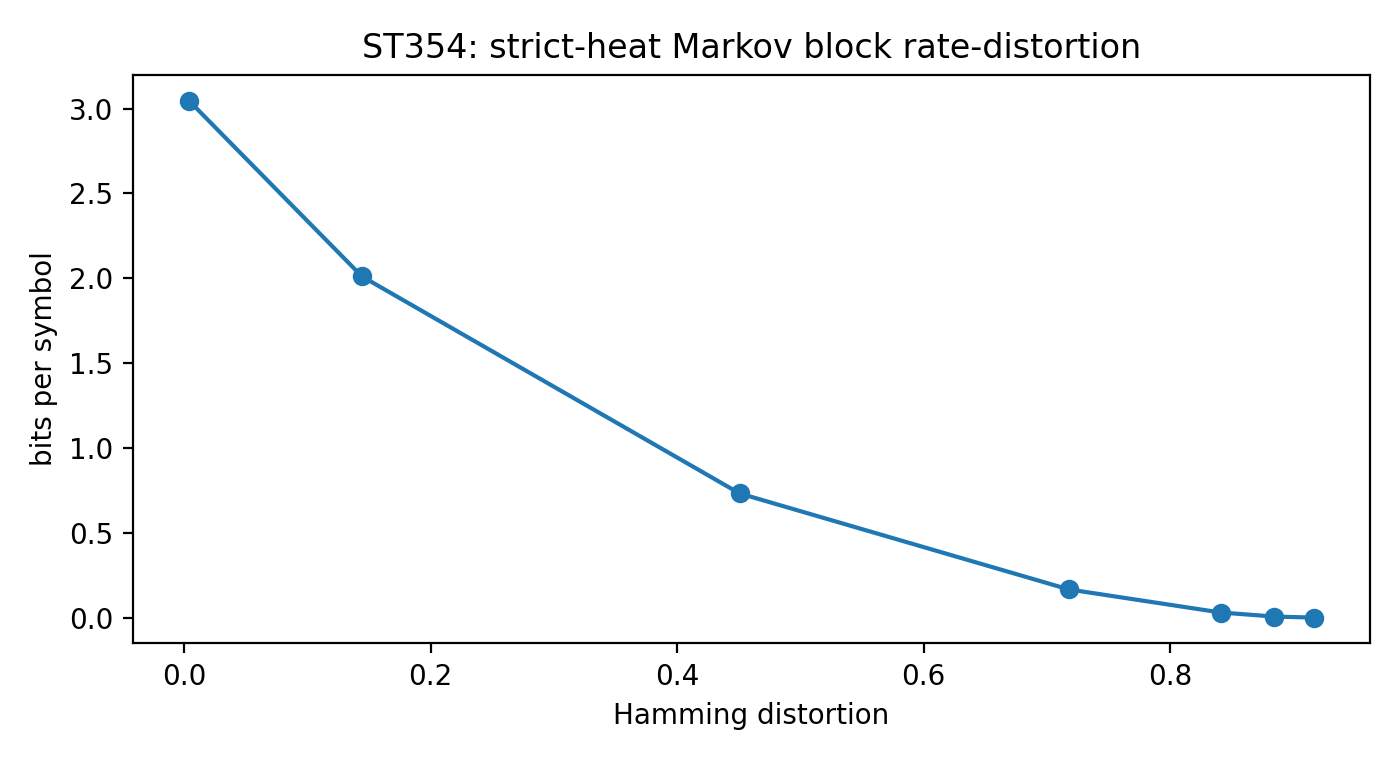
\includegraphics[width=.72\textwidth]{FIN_ST342_ST356_Figures/st354_heat_rate_distortion.png}
\caption{Two-symbol rate--distortion for the conditional strict-heat Markov source.}
\end{figure}

The operator supplies the transition only after the Markov reading and $\tau$ are declared.
It does not identify physical entropy density, bits per volume, or compression of the
universe.

Across several refinement levels, suppose mode $i$ transforms as
\[
\lambda_i^{(n+1)}=c_n\lambda_i^{(n)}(1+\delta_{i,n}),
\qquad |\delta_{i,n}|\le\eta_n<1.
\]
Every common calibration $c_n$ cancels from a modal ratio. Differential unitary/heat clock
drift obeys
\[
\prod_n\frac{1-\eta_n}{1+\eta_n}
\le
\frac{(\lambda_i/\lambda_j)_{N}}{(\lambda_i/\lambda_j)_0}
\le
\prod_n\frac{1+\eta_n}{1-\eta_n},
\]
and wave-clock ratios use square roots. This cleanly separates observer-layer gauge from
real accumulated relative drift, but does not create seconds or an arrow of time.

ST356 applies the empirical stop rule. No independently registered, hashed raw-event file
with separated provider, registrar, and analyst roles exists. Local code cannot generate
that missing fifth measurement obligation.

\section{Falsification ledger and present interpretation}

\begin{longtable}{p{.28\textwidth}p{.28\textwidth}p{.37\textwidth}}
\toprule Proposed conclusion&Falsification test&Surviving statement\\\midrule\endhead
The coexistence location is only a plot&Outward bisection and tube&False: a local crossing lies in a width-$2\times10^{-8}$ interval.\\
The fold remains purely numerical&Full 17D Krawczyk test&False for event existence and nullity; transversality and global dynamics remain open.\\
Dihedral symmetry reduces the global problem&Trivial-stabilizer stratum&False: the generic simplex stratum remains 11-dimensional.\\
The reflection orbit is globally proved&173 starts plus ST344&Still false: strong evidence is not an exhaustive certificate.\\
Any low-rank mediator localizes&Covariant modal truncations&False at $g=4$ through rank five; rank seven is first.\\
Strict invariance uniquely fixes a stabilizer&Quartic/sextic basis count&False: at least 77 coefficients are free in the scoped subalgebra.\\
Filter forgetting closes Chernoff asymptotics&i.i.d. zero-memory control&False: pressure derivatives can persist at zero memory.\\
Anisotropic widths close the branch tube&Outer interval tests&False so far: 34 pass and six fail.\\
Observer depth is only binary&12-state deficiency theorem&False in the symmetric family; the exact depth remains $e_c-e_f$.\\
Compression needs an unrelated source&Strict heat Markov law&Partly false: $e^{-\tau A}$ supplies a conditional source after $\tau$ and the Markov reading are declared.\\
Refinement calibration drift is inseparable&Product theorem&False: common gauge cancels; only differential error accumulates.\\
Local work is physical evidence&Independent record gate&False: ST356 remains blocked.\\
\bottomrule
\end{longtable}

The deepest interpretation surviving this batch is:
\begin{quote}
Once a signed active interaction is supplied, FIN supports a sharply certified local
variational geometry: localized coexistence is known to eight decimal places in the
coupling, and a one-null-direction fold event is isolated in seventeen variables. The
remaining obstacle is genuinely global and source-theoretic, not a lack of local numerical
precision. Dihedral symmetry generates equivalent branches but cannot select or exhaust
them. A sufficiently rich set of strict spectral modes can support localization, while
operational observer depth, conditional compression, scale holonomy, and relative-clock
drift admit exact quantitative laws. None of these laws supplies the active sign, its
magnitude, an absolute unit, or an empirical realization.
\end{quote}

\section{Recommended programs ST357--ST371}

\begin{enumerate}
\item[\textbf{ST357}.] Interval-enclose both fold transversality coefficients and derive the local saddle-node normal form from ST343.
\item[\textbf{ST358}.] Build entropy-convex cell lower bounds for a structure-aware global dual branch-and-bound, avoiding tensor grids.
\item[\textbf{ST359}.] Prove a $D_{12}$ rearrangement theorem for the strict quadratic form or construct an explicit chiral lower-energy counterexample.
\item[\textbf{ST360}.] Conditional on ST358/ST359, certify or refute global $g=4$ minimizer uniqueness modulo $D_{12}$.
\item[\textbf{ST361}.] Interval-certify the rank-seven localized state and compare it globally against uniform and boundary strata.
\item[\textbf{ST362}.] Compute the full Molien series and phase-sensitive degree-four/six $D_{12}$ invariant basis beyond modal energies.
\item[\textbf{ST363}.] Prove a normalized Ruelle/Chernoff pressure-derivative bound for the frozen HMM or isolate a pressure-level counterexample.
\item[\textbf{ST364}.] Implement rotated tangent/transverse interval-Newton slabs and certify a continuous ST298 branch segment.
\item[\textbf{ST365}.] Interval-certify the continuum IR dual multipliers, all threshold zeros, and the corrected two-band optimum.
\item[\textbf{ST366}.] Extend ST352 from permutation-covariant confusion to arbitrary 12-state cyclic convolution instruments by a Fourier LP.
\item[\textbf{ST367}.] Replace the Gaussian fiber model by multinomial child counts and derive finite-sample confidence/minimax bounds.
\item[\textbf{ST368}.] Compute block lengths $3$--$5$ for the strict-heat Markov source and bracket the asymptotic rate--distortion function.
\item[\textbf{ST369}.] Replace worst-case multilevel clock products by martingale/concentration bounds under a declared zero-mean refinement-error law.
\item[\textbf{ST370}.] Admit an active-coupling study only if a genuinely new strict typed source object is supplied; otherwise preserve the existing source no-go.
\item[\textbf{ST371}.] Resume empirical validation only after preregistered independent raw events and separated custody exist.
\end{enumerate}

The highest priority is ST357 because it can convert the certified event into a complete
local simple-fold theorem at low cost. ST358--ST360 address the harder global obstruction.
ST362 and ST363 close clearly identified algebraic and information-theoretic gaps. ST370 is
not permission to replay exhausted selector or bridge searches.

\section{Reproducibility and conclusion}

The executable source \texttt{fin\_st342\_st356\_research.py} writes fifteen program
packets, one aggregate JSON, a CSV ledger, and three figures. The independent suite
\texttt{test\_fin\_st342\_st356.py} performs sixteen live checks covering packet hashes,
interval signs and inclusion, the 17D residual and rank margin, trivial stabilizer,
nonpromotion of the global claim, modal thresholds, invariant counts, the Chernoff
counterexample, incomplete slabs, IR dual normalization, cohomology rank, the full
12-state stochastic LP, sharp risk scaling, the strict-heat Markov law, multilevel drift,
and the evidence stop. All sixteen tests pass.

Release 10.80 makes a real local advance: the phase-transition branch and its fold event
are no longer merely high-quality plots. It simultaneously sharpens the principal negative
conclusion. Better local certification cannot substitute for a global variational theorem
or for the missing source of the active signed coupling. Those are now the two cleanly
separated mathematical frontiers.

\end{document}
